% Created 2015-04-02 Thu 23:07
\documentclass[11pt]{article}
\usepackage[utf8]{inputenc}
\usepackage[T1]{fontenc}
\usepackage{fixltx2e}
\usepackage{graphicx}
\usepackage{longtable}
\usepackage{float}
\usepackage{wrapfig}
\usepackage{soul}
\usepackage{textcomp}
\usepackage{marvosym}
\usepackage{wasysym}
\usepackage{latexsym}
\usepackage{amssymb}
\usepackage{hyperref}
\tolerance=1000
\usepackage{methodshw, amsmath}
\providecommand{\alert}[1]{\textbf{#1}}

\title{8004 Homework 8}
\author{Nooreen Dabbish}
\date{\today}
\hypersetup{
  pdfkeywords={},
  pdfsubject={},
  pdfcreator={Emacs Org-mode version 7.9.3f}}

\begin{document}

\maketitle




\section{This is Problem 3 of Faraway (2006), Chapter 9}
\label{sec-1}


The \verb~ratdrink~ data consist of five weekly measurements of body
weight for 27 rats. The first 10 rats are on a control treatment
while seven rats have thyroxine added to their drinking water. Ten
rats have thiouracil added to their water. Build a model for the rat
weights that shows the effect of the treatment.


\begin{verbatim}
library(faraway)
data(ratdrink)
\end{verbatim}
\subsection{Model the weights of the rate, incorporating the treatment effects and random effect. Use R to fit the model.}
\label{sec-1-1}


We write y$_{\mathrm{ijk}}$ to represent the kth rat in the jth treatment group
on the ith week, where (i=1,2,3,4), (j=1,2,3), and (k= 1-10 for
control, k = 1-7 thyroxine, and k = 1-10 for thiouracil). $\mu$
represents the overall mean weight, $\alpha$$_i$ represents the fixed
effect contribution of the ith week, $\beta$$_j$ repsents the fixed
effect contribution of the jth treatment, and $\delta$$_{\mathrm{ij}}$ is the
interaction of weeks and treatment. The random effect u$_{\mathrm{jk}}$
incorporates the repeated measures of the same rat.

$$y_{ijk} = \mu + \alpha_i + \beta_j + \delta_{ij} + u_{jk} + \epsilon_{ijk}$$

To fit the model in R we write:

 \verb,rat.lme <- lmer(wt ~ weeks+ treat+ weeks*treat+ (1|subject)),

The command \verb~summary(rat.lme)~ gives:

\begin{verbatim}
Linear mixed model fit by REML ['lmerMod']
Formula: wt ~ weeks + treat + weeks * treat + (1 | subject)

REML criterion at convergence: 948.4

Scaled residuals: 
     Min       1Q   Median       3Q      Max 
-2.05506 -0.65511 -0.04848  0.57702  2.80847 

Random effects:
 Groups   Name        Variance Std.Dev.
 subject  (Intercept) 71.21    8.438   
 Residual             51.22    7.157   
Number of obs: 135, groups:  subject, 27

Fixed effects:
                      Estimate Std. Error t value
(Intercept)            52.8800     3.1928   16.56
weeks                  26.4800     0.7157   37.00
treatthiouracil         4.7800     4.5153    1.06
treatthyroxine         -0.7943     4.9756   -0.16
weeks:treatthiouracil  -9.3700     1.0121   -9.26
weeks:treatthyroxine    0.6629     1.1153    0.59

Correlation of Fixed Effects:
            (Intr) weeks  trtthr trtthy wks:trtthr
weeks       -0.448                                
treatthircl -0.707  0.317                         
treatthyrxn -0.642  0.288  0.454                  
wks:trtthrc  0.317 -0.707 -0.448 -0.203           
wks:trtthyr  0.288 -0.642 -0.203 -0.448  0.454    
\end{verbatim}
\subsection{What is the implication of the random effect on the correlations between weights of the same rat? Is that implication reasonable? It would be nice to support your argument with data evidence.}
\label{sec-1-2}


The random effect captures the correlation between measuring the same
rat on multiple weeks. Because that rat has a starting weight at week
zero, subsequent measurements will be correlated with the previous weight.
 
We fit a completely fixed model and call \verb~summary(rat.lm)~ for
comparison. As shown below, and as we would expect, 
the fixed coefficient estimates are the same without the random
effect from the same rat. However, above, we were able to obtain a
correlation matrix showing the correlation of the fixed effects. The
correlation across weeks for the overall mean obtained was -.448,
which is relatively low (highly correlated would be close to 1, or
inversely correlated close to -1). 

\begin{verbatim}
> rat.lm <- lm(wt ~weeks+treat+weeks*treat)
> summary(rat.lm)

Call:
lm(formula = wt ~ weeks + treat + weeks * treat)

Residuals:
    Min      1Q  Median      3Q     Max 
-23.514  -6.660   0.230   6.914  28.343 

Coefficients:
                      Estimate Std. Error t value Pr(>|t|)    
(Intercept)            52.8800     2.6547  19.919  < 2e-16 ***
weeks                  26.4800     1.0838  24.433  < 2e-16 ***
treatthiouracil         4.7800     3.7544   1.273    0.205    
treatthyroxine         -0.7943     4.1371  -0.192    0.848    
weeks:treatthiouracil  -9.3700     1.5327  -6.113 1.08e-08 ***
weeks:treatthyroxine    0.6629     1.6890   0.392    0.695    
---
Signif. codes:  0 ‘***’ 0.001 ‘**’ 0.01 ‘*’ 0.05 ‘.’ 0.1 ‘ ’ 1

Residual standard error: 10.84 on 129 degrees of freedom
Multiple R-squared:  0.9121,    Adjusted R-squared:  0.9087 
F-statistic: 267.8 on 5 and 129 DF,  p-value: < 2.2e-16
\end{verbatim}
\section{The article “Variability of Sliver Weights at Different Carding Stages and a Suggested Sampling Plan for Jute Processing”}
\label{sec-2}

by A. Lahiri (Journal of the Textile Institute, 1990) concerns the 
partitioning
of variability in “sliver weight.” (A sliver is a continuous strand
of loose, untwisted wool, cotton,
etc., produced along the way to making yarn.) For a particular mill, 
3 (of many) machines were
studied, using 5 (10 mm) pieces of sliver cut from each of 5 rolls produced on the machines. The
weights of the (75) pieces of sliver were determined and a standard hierarchical (balanced data)
ANOVA table was produced as below. (The units of weight were not given in the original article.)


\begin{center}
\begin{tabular}{lrr}
 Source    &    SS  &  df  \\
\hline
 Machines  &  1966  &   2  \\
 Rolls     &   644  &  12  \\
 Pieces    &   280  &  60  \\
\hline
 Total     &  2890  &  74  \\
\end{tabular}
\end{center}




The model is $$y_{ijk} = \mu + \alpha_i +u_{ij} + \epsilon_{ijk}$$

for the kth piece of the jth roll on the ith machine, where
$$\alpha_i \overset{iid}{\sim} N(0,\sigma^2_\alpha), \,
u_{ij} \overset{iid}{\sim} N(0,\sigma^2_u), \text{and}\, 
\epsilon_i \overset{iid}{\sim} N(0,\sigma^2_\epsilon).$$  
\subsection{Find estimates for $\sigma$$^2$$_{\alpha}$, $\sigma$$^2$$_u$ and $\sigma$$^2$$_{\epsilon}$.}
\label{sec-2-1}



\begin{center}
\begin{tabular}{lrrllrl}
 Source    &    SS  &  df  &  Term   &  MS     &             &  E(MS)                                              \\
\hline
 Machines  &  1966  &   2  &         &  MSA    &        983  &  \sigma^2_\epsilon + 5\sigma^2_u+25\sigma^2_\alpha  \\
 Rolls     &   644  &  12  &         &  MSB]A  &  53.666667  &  \sigma^2_\epsilon + 5\sigma^2_u                    \\
 Pieces    &   280  &  60  &  error  &  MSE    &  4.6666667  &  \sigma^2_\epsilon                                  \\
\hline
 Total     &  2890  &  74  &         &         &             &                                                     \\
\end{tabular}
\end{center}



Solving for the expectations above gives the following estimates:

\begin{itemize}
\item $\widehat{\sigma^2_{\epsilon}} = 4.6667$
\item $\widehat{\sigma^2_u} = 9.8$
\item $\widehat{\sigma^2_{\alpha}} = 37.17333$
\end{itemize}
\subsection{Make 95\% confidence intervals for each of the 3 standard deviations}
\label{sec-2-2}

$\sigma$$_{\alpha}$, $\sigma$$_u$, and $\sigma$$_{\epsilon}$.
Based on theses, where do you judge the largest part of the variation
in measured weight to come from? You need to use the
Cochran-Satterthwaite approximation for $\sigma$$_{\alpha}$ and $\sigma$$_u$.

For $\sigma$$_{\epsilon}$ we note that 
$$\frac{SSE}{\sigma_{\epsilon}} \sim \chi^2_{60}.$$ 

We write:

$$c(\sigma_{\epsilon}) = \left( \sigma_{\epsilon} : \chi^2_{60,.05} < \frac{SSE}{\sigma^2_{\epsilon}} < \chi^2_{60,.95} \right)$$
$$c(\sigma_{\epsilon}) = \left( \sigma_{\epsilon} : \sqrt{\frac{SSE}{\chi^2_{60,.95}}} < \sigma_{\epsilon} < \sqrt{\frac{SSE}{\chi^2_{60,.05}}} \right)$$
$$c(\sigma_{\epsilon}) = \left( \sigma_{\epsilon} : 1.833423 <
\sigma_{\epsilon} < 2.629961 \right)$$

We use the Cochran-Satterwaithe approximation for $\sigma$_$\alpha$ and
$\sigma$$_u$. There \hat{v} is used to determine the degrees of freedom
of a Chi-squared distribution which is approximately:

$$\frac{v(S^2)}{E(S^2)} \sim \chi^2_v$$

This gives us a 1-$\alpha$ confidence interval for E(S$^2$) determined by:

$$P\left( \frac{v \cdot S^2}{\chi^2_{v,upper}} < E(S^2) < \frac{v \cdot S^2}{\chi^2_{v,lower}} \right)=1-\alpha$$

$$\hat{v}_u =
\frac{(\sigma^2_u)^2}{\frac{((MSB|A)/5)^2}{df=12}+\frac{(-MSE/5)^2}{df=60}}
= 9.988675$$

$$\hat{v}_\alpha =
\frac{(\sigma^2_\alpha)^2}{\frac{((-MSB|A)/25)^2}{df=12}+\frac{(MSA/25)^2}{df=2}}
= 1.786695$$

Solving for our confidence intervals gives 
$$c(\sigma_u) = (\sigma_u : 2.186967 < \sigma_u < 5.496051)$$
$$c(\sigma_\alpha) = (\sigma_\alpha : 3.097864 < \sigma_\alpha < 46.29789)$$

Clearly, the largest contribution to the variability in the measured
weight of the silver comes from the differences between machines.
This is because the estimate of the standard deviation associated
with $\sigma$_$\alpha$ isthe largest, and its confidence interval also
ranges over the largest values.
\subsection{Suppose for the sake of illustration that the grand average}
\label{sec-2-3}

of all 75 weight measurements was in fact $\bar{y_\ldots}$ = 1/75
$\sum$$_{\mathrm{ijk}}$ y$_{\mathrm{ijk}}$ = 35.0.\$ Use this and information from the ANOVA
table to make a 95\% confidence interval for the model parameter $\mu$.

The 95\% confidence interval we are interested in is $\bar{y_\ldots}$
\textpm{} t$_{\mathrm{.975,df=2}}$ \sqrt{\frac{MSA}{3\cdot 5\cdot 5}} = (19.42305,50.57695).
\section{Appendix: Tangled R Code}
\label{sec-3}


\lstinputlisting{DabbishHW8.R} 
\section{Appendix: Initial evaluation of ratdrink dataset}
\label{sec-4}


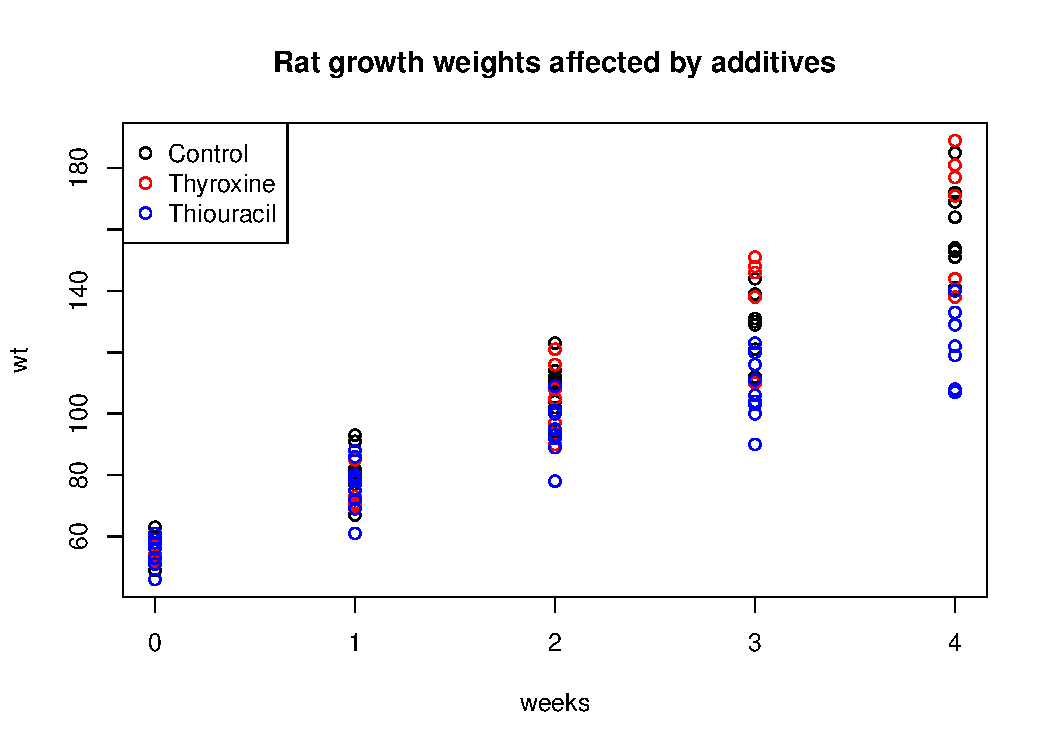
\includegraphics[width=.9\linewidth]{./ratweights.pdf}

Plotting the ratdrink data suggested that rats that drank Thyroxine
tended to have increased body weight after 5 weeks in comparison to rats
drinking Thiouracil and Control. The rats that drank Thiouracil
tended to have lowerbody weight than the Control and Thyroxine groups.

\end{document}
